\documentclass[aspectratio=169,11pt]{beamer}

\usetheme{Madrid}
\usecolortheme{default}
\usefonttheme{professionalfonts}

\usepackage[T1]{fontenc}
\usepackage{lmodern}
\usepackage{booktabs}
\usepackage{array}
\usepackage{pgfplots}
\usepackage{xcolor}
\usepackage{listings}

\pgfplotsset{compat=1.18}

\definecolor{nsblue}{RGB}{28,93,153}
\definecolor{nsgreen}{RGB}{26,130,90}
\definecolor{nsorange}{RGB}{210,120,30}
\definecolor{nsred}{RGB}{185,55,55}
\definecolor{softgray}{RGB}{245,246,248}

\setbeamercolor{structure}{fg=nsblue}
\setbeamercolor{frametitle}{fg=white,bg=nsblue}
\setbeamercolor{title}{fg=white,bg=nsblue}
\setbeamerfont{title}{size=\Large,series=\bfseries}
\setbeamerfont{frametitle}{size=\Large,series=\bfseries}
\setbeamerfont{normal text}{size=\normalsize}
\setbeamertemplate{navigation symbols}{}
\setbeamertemplate{itemize items}[circle]

\lstset{
  basicstyle=\ttfamily\footnotesize,
  backgroundcolor=\color{softgray},
  frame=single,
  breaklines=true,
  columns=fullflexible
}

\title[PRR Density Analysis]{NR-V2X PRR Analysis Under Vehicle Density}
\subtitle{Simulation Upgrades, Results, Interpretation, and Next Steps}
\author{Prepared for Professor}
\institute{ns-3 NR-V2X / DeePC Dataset Study}
\date{\today}

\begin{document}

\begin{frame}
  \titlepage
\end{frame}

\begin{frame}{Presentation Goal}
\large
\begin{itemize}
  \item Explain what was changed in the ns-3 NR-V2X simulation.
  \item Show how PRR changes when vehicle density is reduced.
  \item Compare our PRR behavior with expected validation behavior.
  \item Identify the most likely reason for low PRR.
  \item Propose the next experiments needed before DeePC dataset generation.
\end{itemize}
\end{frame}

\begin{frame}[fragile]{Experimental Context}
\large
\begin{itemize}
  \item Mobility source: processed NGSIM US-101 trajectory CSV.
  \item Loaded vehicles in CSV: \textbf{54 unique vehicle IDs}.
  \item Simulation can now select fewer vehicles using:
\end{itemize}

\vspace{0.3cm}
\begin{lstlisting}
--maxVehicles=5
--maxVehicles=10
--maxVehicles=54
\end{lstlisting}

\vspace{0.2cm}
\large
\begin{itemize}
  \item This allows PRR analysis as a function of vehicle density.
\end{itemize}
\end{frame}

\begin{frame}{Main Simulation Upgrades}
\large
\begin{itemize}
  \item Added exact PRR logging using TX-time eligibility.
  \item Added per-distance-bin TX denominators:
  \[
    0-50,\quad 50-100,\quad 100-150,\quad 150-200,\quad 200-300 \text{ m}
  \]
  \item Added runtime Tx power updates at the UE PHY.
  \item Added real CBR logging from NR spectrum busy-time traces.
  \item Added vehicle count control with \texttt{--maxVehicles}.
  \item Added fixed-input validation mode with \texttt{--useInputSchedule=false}.
\end{itemize}
\end{frame}

\begin{frame}{PRR Definition Used}
\large
For each transmission event \(j\):

\[
E_j(d \in [a,b]) =
\text{number of receivers in distance bin at TX time}
\]

\[
R_j(d \in [a,b]) =
\text{number of successful receptions in that bin}
\]

\[
\mathrm{PRR}_{[a,b]} =
\frac{\sum_j R_j(d \in [a,b])}
     {\sum_j E_j(d \in [a,b])}
\]

\vspace{0.2cm}
\begin{block}{Why this matters}
The denominator now comes from eligible receivers at transmission time, not from already-received packets.
\end{block}
\end{frame}

\begin{frame}{Validation Reference Behavior}
\large
Expected PRR-vs-distance behavior from reference-style NR-V2X plots:

\vspace{0.25cm}
\begin{itemize}
  \item PRR close to \(0.95-1.0\) at short range.
  \item PRR decreases smoothly with Tx-Rx distance.
  \item PRR remains around \(0.5-0.6\) even near 500 m in the reference case.
\end{itemize}

\vspace{0.3cm}
\begin{block}{Our target}
Our curve should be high at short distance and should degrade gradually as distance increases.
\end{block}
\end{frame}

\begin{frame}{Vehicle Density Experiments}
\large
I tested PRR after reducing the number of simulated vehicles:

\vspace{0.25cm}
\begin{table}
\centering
\renewcommand{\arraystretch}{1.25}
\begin{tabular}{>{\raggedright}p{3.2cm} >{\raggedright}p{3.6cm} >{\raggedright\arraybackslash}p{4.2cm}}
\toprule
\textbf{Case} & \textbf{Purpose} & \textbf{Observation} \\
\midrule
54 vehicles & Original dense case & Very low PRR \\
10 vehicles & Reduced density & PRR improved strongly \\
5 vehicles & Low-density case & PRR improved, but still not near 1 \\
5 vehicles fixed input & Remove PRBS mixing & PRR stayed almost same \\
\bottomrule
\end{tabular}
\end{table}
\end{frame}

\begin{frame}{PRR Results by Distance}
\small
\begin{table}
\centering
\renewcommand{\arraystretch}{1.25}
\begin{tabular}{lccccc}
\toprule
\textbf{Vehicles} & \textbf{25 m} & \textbf{75 m} & \textbf{125 m} & \textbf{175 m} & \textbf{250 m} \\
\midrule
54 & 0.125 & 0.063 & 0.067 & 0.031 & 0.021 \\
10 & 0.510 & 0.450 & 0.405 & 0.470 & 0.220 \\
5 & 0.600 & 0.482 & -- & -- & 0.414 \\
5 fixed input & 0.600 & 0.482 & -- & -- & 0.414 \\
\bottomrule
\end{tabular}
\end{table}

\vspace{0.25cm}
\footnotesize
Values are approximate from the generated PRR-vs-distance plots.
\end{frame}

\begin{frame}{PRR vs Distance Plot}
\centering
\begin{tikzpicture}
\begin{axis}[
    width=0.86\textwidth,
    height=0.58\textheight,
    xlabel={TX-time distance bin center (m)},
    ylabel={PRR},
    xmin=0, xmax=275,
    ymin=0, ymax=0.70,
    grid=both,
    legend style={at={(0.98,0.98)},anchor=north east,font=\footnotesize},
    tick label style={font=\small},
    label style={font=\small}
]
\addplot[color=nsred,mark=*] coordinates {
    (25,0.125) (75,0.063) (125,0.067) (175,0.031) (250,0.021)
};
\addlegendentry{54 vehicles}

\addplot[color=nsorange,mark=square*] coordinates {
    (25,0.510) (75,0.450) (125,0.405) (175,0.470) (250,0.220)
};
\addlegendentry{10 vehicles}

\addplot[color=nsgreen,mark=triangle*] coordinates {
    (25,0.600) (75,0.482) (250,0.414)
};
\addlegendentry{5 vehicles}

\addplot[color=nsblue,mark=diamond*,dashed] coordinates {
    (25,0.600) (75,0.482) (250,0.414)
};
\addlegendentry{5 vehicles fixed input}
\end{axis}
\end{tikzpicture}
\end{frame}

\begin{frame}{Key Observation 1: Density Matters}
\large
\begin{itemize}
  \item Reducing vehicles from 54 to 10 increased short-range PRR from about \(0.125\) to about \(0.51\).
  \item Reducing to 5 vehicles increased short-range PRR to about \(0.60\).
  \item This strongly suggests that the dense case suffers from congestion and resource collisions.
\end{itemize}

\vspace{0.25cm}
\begin{block}{Conclusion}
The original low PRR is not only a pathloss problem. Vehicle density and sidelink resource contention are major factors.
\end{block}
\end{frame}

\begin{frame}{Key Observation 2: Fixed Input Did Not Improve PRR}
\large
The fixed-input test used:

\[
P = 23 \text{ dBm}, \quad T_b = 0.1 \text{ s}
\]

\vspace{0.2cm}
\begin{itemize}
  \item PRBS schedule was disabled.
  \item Tx power and beacon interval were kept constant.
  \item The 5-vehicle PRR curve stayed almost unchanged.
\end{itemize}

\vspace{0.25cm}
\begin{block}{Conclusion}
Low PRR is probably not caused mainly by PRBS input mixing.
\end{block}
\end{frame}

\begin{frame}{Key Observation 3: MCS Change Did Not Help}
\large
I also tested lower MCS:

\[
\mathrm{MCS}=10 \quad \rightarrow \quad \mathrm{MCS}=6
\]

\vspace{0.2cm}
\begin{itemize}
  \item PRR remained almost the same.
  \item This suggests that packet loss is not mainly due to modulation/coding robustness.
\end{itemize}

\vspace{0.25cm}
\begin{block}{Interpretation}
The next suspects are resource collisions, sidelink resource configuration, groupcast reception behavior, or vehicle geometry.
\end{block}
\end{frame}

\begin{frame}{Current Diagnosis}
\large
\begin{table}
\centering
\renewcommand{\arraystretch}{1.25}
\begin{tabular}{p{5.0cm} p{6.4cm}}
\toprule
\textbf{Evidence} & \textbf{Meaning} \\
\midrule
PRR improves when vehicles decrease & Congestion/resource collision is important \\
5 vehicles still only about 0.6 PRR near 25 m & Another issue remains \\
Fixed input gives same PRR & PRBS mixing is not the main cause \\
MCS 6 gives same PRR as MCS 10 & PHY coding robustness is not the main cause \\
\bottomrule
\end{tabular}
\end{table}
\end{frame}

\begin{frame}{Most Likely Remaining Causes}
\large
\begin{enumerate}
  \item Sidelink resource selection or sensing configuration.
  \item Resource pool too small or poorly matched to the traffic.
  \item First selected vehicle IDs may still be spatially clustered.
  \item Groupcast bearer or receive filtering may not match all eligible receiver pairs.
  \item Warm-up or transient effects may still be included in some plots.
  \item Need a two-vehicle sanity test to isolate PHY/MAC behavior.
\end{enumerate}
\end{frame}

\begin{frame}[fragile]{Next Step 1: Two-Vehicle Sanity Test}
\large
Run the cleanest possible test:

\begin{lstlisting}
./ns3 run "scratch/nr_v2x_ngsim_deepc \
  --maxVehicles=2 \
  --useInputSchedule=false \
  --txPower=23 \
  --fixedBeaconInterval=0.5 \
  --mcs=6 \
  --simTime=60 \
  --warmup=10 \
  --kpiCsv=data/output/kpi_2veh_tb05.csv"
\end{lstlisting}

\vspace{0.2cm}
\begin{block}{Expected interpretation}
If PRR is near 1, the PHY/bearer path is fine. If PRR stays near 0.5, there is a deeper configuration or logging problem.
\end{block}
\end{frame}

\begin{frame}{Next Step 2: Beacon Interval Sweep}
\large
Test whether traffic load is still causing collisions:

\[
T_b \in \{0.1,\ 0.2,\ 0.5,\ 1.0\}\text{ s}
\]

\vspace{0.3cm}
\begin{itemize}
  \item If PRR improves as \(T_b\) increases, load/collision is the dominant issue.
  \item If PRR does not improve, the issue is likely resource configuration, groupcast reception, or accounting.
\end{itemize}
\end{frame}

\begin{frame}[fragile]{Next Step 3: Sensing On/Off Comparison}
\large
Compare:

\begin{lstlisting}
--enableSensing=true
--enableSensing=false
\end{lstlisting}

\vspace{0.25cm}
\begin{itemize}
  \item If sensing improves PRR, collisions are likely and sensing helps.
  \item If sensing reduces PRR, sensing parameters may be poorly configured.
  \item If both are similar, the issue may be elsewhere.
\end{itemize}
\end{frame}

\begin{frame}[fragile]{Next Step 4: Vehicle Selection Method}
\large
Current selection:

\begin{lstlisting}
--maxVehicles=5
\end{lstlisting}

takes the first sorted vehicle IDs.

\vspace{0.25cm}
\begin{itemize}
  \item These vehicles may be spatially clustered.
  \item Next improvement: add random or spacing-aware vehicle selection.
  \item This helps separate density effects from geometry effects.
\end{itemize}
\end{frame}

\begin{frame}{Decision Tree}
\large
\begin{table}
\centering
\renewcommand{\arraystretch}{1.25}
\begin{tabular}{p{5.2cm} p{6.2cm}}
\toprule
\textbf{Test Result} & \textbf{Conclusion} \\
\midrule
2 vehicles PRR near 1 & PHY/bearer okay; collision/load is the issue \\
2 vehicles PRR near 0.5 & Check sidelink config, groupcast, or logging \\
PRR improves with larger \(T_b\) & Offered load is too high \\
PRR unchanged with larger \(T_b\) & Resource/bearer/accounting issue likely \\
Sensing off improves PRR & Sensing config may be hurting selection \\
\bottomrule
\end{tabular}
\end{table}
\end{frame}

\begin{frame}{Summary}
\large
\begin{itemize}
  \item I upgraded the simulation to support exact PRR-vs-distance validation.
  \item I added vehicle-density control and fixed-input validation mode.
  \item Reducing vehicles greatly improves PRR.
  \item However, 5 vehicles still gives only about 0.6 PRR at short distance.
  \item PRBS mixing and MCS are not the main causes.
  \item Next work: two-vehicle sanity test, beacon interval sweep, sensing on/off, and vehicle selection analysis.
\end{itemize}
\end{frame}

\begin{frame}{Final Message}
\centering
\Large
The simulation now shows that vehicle density strongly affects PRR, but a remaining baseline loss issue must be isolated before building the final DeePC dataset.

\vspace{0.6cm}
\large
Next target: prove whether the remaining loss comes from resource collisions or from sidelink configuration.
\end{frame}

\end{document}
